\documentclass[tikz,border=8pt]{standalone}
\usetikzlibrary{arrows.meta,shapes.geometric}
\definecolor{bg}{HTML}{FAFBFD}
\definecolor{offline}{HTML}{F3F0FA}
\definecolor{offlineedge}{HTML}{7B5EA7}
\definecolor{online}{HTML}{EAF4FB}
\definecolor{onlineedge}{HTML}{2A6F97}
\definecolor{doc}{HTML}{FFF4DC}
\definecolor{docedge}{HTML}{C98A1B}
\definecolor{vec}{HTML}{E3F2EA}
\definecolor{vecedge}{HTML}{2E7D4F}
\definecolor{llm}{HTML}{FDE7E7}
\definecolor{llmedge}{HTML}{C0392B}
\definecolor{ink}{HTML}{233044}
\definecolor{sig}{HTML}{3A3F47}
\begin{document}
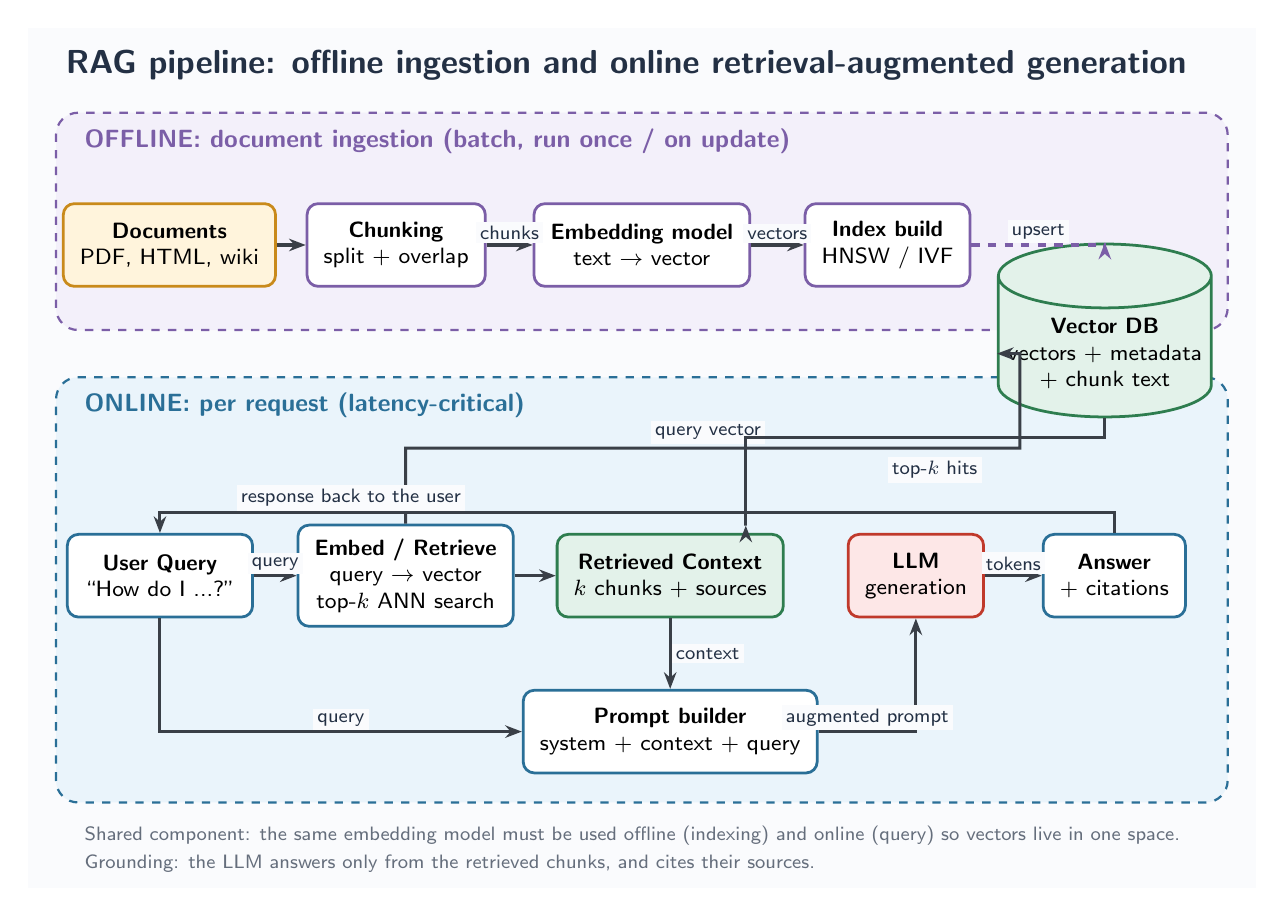
\begin{tikzpicture}[x=1.2cm,y=1.2cm,font=\sffamily\footnotesize,
  box/.style={draw,line width=1pt,rounded corners=4pt,align=center,inner xsep=6pt,inner ysep=5pt,minimum height=1.05cm},
  flow/.style={-{Stealth[length=6pt]},line width=1.1pt,sig},
  off/.style={-{Stealth[length=6pt]},line width=1.1pt,offlineedge,dashed},
  lbl/.style={font=\sffamily\scriptsize,text=ink,fill=bg,inner sep=1.5pt},
  sub/.style={font=\sffamily\scriptsize,text=ink!70!white}]
  \fill[bg] (-0.6,-0.7) rectangle (12.4,8.4);
  \node[font=\sffamily\bfseries\large,text=ink,anchor=west] at (-0.3,8.0) {RAG pipeline: offline ingestion and online retrieval-augmented generation};

  % ===== lanes =====
  \fill[offline,rounded corners=8pt] (-0.3,5.2) rectangle (12.1,7.5);
  \draw[offlineedge,dashed,line width=0.8pt,rounded corners=8pt] (-0.3,5.2) rectangle (12.1,7.5);
  \node[font=\sffamily\bfseries\small,text=offlineedge,anchor=west] at (-0.1,7.2) {OFFLINE: document ingestion (batch, run once / on update)};
  \fill[online,rounded corners=8pt] (-0.3,0.2) rectangle (12.1,4.7);
  \draw[onlineedge,dashed,line width=0.8pt,rounded corners=8pt] (-0.3,0.2) rectangle (12.1,4.7);
  \node[font=\sffamily\bfseries\small,text=onlineedge,anchor=west] at (-0.1,4.4) {ONLINE: per request (latency-critical)};

  % ===== offline row =====
  \node[box,draw=docedge,fill=doc] (docs) at (0.9,6.1) {\textbf{Documents}\\PDF, HTML, wiki};
  \node[box,draw=offlineedge,fill=white] (chunk) at (3.3,6.1) {\textbf{Chunking}\\split + overlap};
  \node[box,draw=offlineedge,fill=white] (embed1) at (5.9,6.1) {\textbf{Embedding model}\\text $\to$ vector};
  \node[box,draw=offlineedge,fill=white] (index) at (8.5,6.1) {\textbf{Index build}\\HNSW / IVF};
  \draw[flow] (docs) -- (chunk);
  \draw[flow] (chunk) -- (embed1) node[lbl,midway,above] {chunks};
  \draw[flow] (embed1) -- (index) node[lbl,midway,above] {vectors};

  % ===== vector DB (shared, cylinder) =====
  \node[cylinder,shape border rotate=90,draw=vecedge,fill=vec,line width=1pt,minimum width=2.7cm,minimum height=2.0cm,aspect=0.3,align=center] (vdb) at (10.8,4.95) {\textbf{Vector DB}\\vectors + metadata\\+ chunk text};
  \draw[off] (index.east) -| (vdb.north) node[lbl,pos=0.25,above] {upsert};

  % ===== online row =====
  \node[box,draw=onlineedge,fill=white] (user) at (0.8,2.6) {\textbf{User Query}\\``How do I ...?''};
  \node[box,draw=onlineedge,fill=white] (embed2) at (3.4,2.6) {\textbf{Embed / Retrieve}\\query $\to$ vector\\top-$k$ ANN search};
  \node[box,draw=vecedge,fill=vec] (ctx) at (6.2,2.6) {\textbf{Retrieved Context}\\$k$ chunks + sources};
  \node[box,draw=onlineedge,fill=white] (prompt) at (6.2,0.95) {\textbf{Prompt builder}\\system + context + query};
  \node[box,draw=llmedge,fill=llm] (llm) at (8.8,2.6) {\textbf{LLM}\\generation};
  \node[box,draw=onlineedge,fill=white] (ans) at (10.9,2.6) {\textbf{Answer}\\+ citations};

  \draw[flow] (user) -- (embed2) node[lbl,midway,above] {query};
  \draw[flow] (embed2.north) -- ++(0,0.0) |- (9.9,3.95) -- (9.9,4.95) -- (vdb.west) ;
  \node[lbl] at (6.6,4.12) {query vector};
  \draw[flow] (vdb.south) -- ++(0,-0.2) -| (7.0,3.6) -- (7.0,3.6) |- (7.0,3.13) ;
  \node[lbl] at (9.0,3.72) {top-$k$ hits};
  \draw[flow] (embed2) -- (ctx);
  \draw[flow] (ctx) -- (prompt) node[lbl,midway,right] {context};
  \draw[flow] (user.south) |- (prompt.west) node[lbl,pos=0.75,above] {query};
  \draw[flow] (prompt.east) -| (llm.south) node[lbl,pos=0.25,above] {augmented prompt};
  \draw[flow] (llm) -- (ans) node[lbl,midway,above] {tokens};
  \draw[flow] (ans.north) -- ++(0,0.22) -| (user.north) node[lbl,pos=0.4,above] {response back to the user};

  % ===== notes =====
  \node[sub,anchor=west] at (-0.1,-0.15) {Shared component: the same embedding model must be used offline (indexing) and online (query) so vectors live in one space.};
  \node[sub,anchor=west] at (-0.1,-0.45) {Grounding: the LLM answers only from the retrieved chunks, and cites their sources.};
\end{tikzpicture}
\end{document}
